% =====================================================================
%  ICASSP 2027 -- rascunho v1
%
%  COMO TROCAR PARA O TEMPLATE OFICIAL DO ICASSP:
%  Baixe o kit do ICASSP (spconf.sty + IEEEbib.bst) e troque as 3 linhas
%  marcadas com  %<<TEMPLATE>>  abaixo. O corpo do texto não muda.
%
%  Compilar: latexmk -pdf main.tex     (ou: pdflatex; bibtex; pdflatex x2)
%  Tabelas e números: gerados por make_tables.py a partir de ../results/*.csv.
%  NÃO edite tables/*.tex à mão -- rode make_tables.py de novo.
% =====================================================================
\documentclass[conference,10pt]{IEEEtran}          %<<TEMPLATE>> -> \documentclass{article}+\usepackage{spconf}
\usepackage[T1]{fontenc}
\usepackage[utf8]{inputenc}
\usepackage{graphicx,amsmath,amssymb,booktabs,xspace,microtype}
\usepackage{siunitx}
\usepackage{xcolor}
\usepackage[hidelinks]{hyperref}
\usepackage{cite}

% GERADO POR make_tables.py -- NAO EDITAR A MAO
\newcommand{\gapGrouped}{+0.046\xspace}
\newcommand{\gapLolo}{-0.146\xspace}
\newcommand{\gapLoloWorst}{-0.453\xspace}
\newcommand{\covEighty}{55\xspace}
\newcommand{\covZero}{0.408\xspace}
\newcommand{\covTwo}{0.729\xspace}
\newcommand{\covFour}{0.522\xspace}
\newcommand{\gateDelta}{-0.003 \pm 0.015\xspace}
\newcommand{\recalFive}{+0.002\xspace}
\newcommand{\recalThreeT}{-0.048\xspace}
\newcommand{\recalThreeST}{-0.099\xspace}   % \gapLolo, \covEighty, ... -- gerados dos CSVs

% Deixa \TODO{} vermelho no rascunho. Para a versão final, troca o corpo
% por {} e todos os lembretes somem sem precisar caçá-los um a um.
\newcommand{\TODO}[1]{\textcolor{red}{\textbf{[TODO: #1]}}}

\title{Calibrate Where You Deploy: Conformal Sensor Escalation\\
       Under Operating-Point Shift}

\author{\IEEEauthorblockN{Cândido de Lucena Filho}
\IEEEauthorblockA{Escola Politécnica, Universidade de São Paulo\\
São Paulo, Brazil\\
\TODO{e-mail, coautores, e o agradecimento de fomento}}}

\begin{document}
\maketitle

% =====================================================================
\begin{abstract}
Condition-monitoring nodes must decide, window by window, whether the
cheap always-on sensor suffices or the expensive acquisition chain has to
be woken. That decision is normally driven by a softmax threshold
$\tau$ with no operational meaning. We replace it with a split-conformal
gate: escalate iff the prediction set is not a singleton. The risk level
$\alpha$ then becomes a specification, and the escalation rate --- hence
the energy bill --- becomes a \emph{measured consequence} rather than a
second tuned knob. On the KAIST bearing dataset (45 recordings, 5 classes,
3 torque loads) we report three results. First, at matched escalation rate
the conformal gate is statistically indistinguishable from the softmax
threshold in accuracy ($\Delta$ macro-F1 $= \gateDelta$); its value is
specification, not accuracy. Second, the coverage guarantee holds under
recording-grouped validation ($\gapGrouped$) but collapses under load
shift ($\gapLolo$ mean, $\gapLoloWorst$ worst case: a nominal 80\% delivers
\covEighty\%). Third, \emph{five} recordings from the target operating
point restore nominal coverage --- and discarding the source calibration
set beats pooling it.
\end{abstract}

\begin{IEEEkeywords}
conformal prediction, condition monitoring, multimodal sensing, TinyML,
distribution shift
\end{IEEEkeywords}

% =====================================================================
\section{Introduction}

% --- CÂNDIDO: este parágrafo é o gancho. Reescreve na tua voz.
Battery-powered condition-monitoring nodes are dominated, energetically, by
their analog front ends. A MEMS accelerometer sampled at
\SI{25.6}{\kilo\hertz} together with its conditioning chain and
high-rate ADC costs orders of magnitude more than a current transformer
sampled slowly, and both cost more than the microcontroller cycles spent
classifying the resulting window. The standard response is a
\emph{cascade}: run a cheap always-on model, and wake the expensive chain
only when the cheap model looks uncertain~\cite{TODOcascade}.

The trouble is the wake-up rule. In practice it is a threshold on the
softmax output, $\max_y \hat p(y \mid x) < \tau$, with $\tau$ swept until
the accuracy--energy trade-off looks acceptable. This is unsatisfying for
two reasons. Softmax scores of small discriminative models are not
calibrated probabilities, so $\tau$ has no units and no operational
meaning; and because $\tau$ is tuned, the escalation rate --- the quantity
that actually sets battery life --- is an outcome of tuning rather than
something the integrator specifies.

Split conformal prediction~\cite{papadopoulos2002,vovk2005,lei2018,angelopoulos2023}
offers a different handle. Given a held-out calibration set and a target
risk $\alpha$, it returns prediction \emph{sets} with finite-sample
marginal coverage $\mathbb{P}(Y \in C(X)) \geq 1-\alpha$ under
exchangeability, with no assumption on the underlying model. We use the
set itself as the gate: escalate iff $|C(x)| \neq 1$. The knob is now
$\alpha$, a risk the integrator states, and the escalation rate is
measured.

% --- CÂNDIDO: a lista de contribuições é o que o revisor lê primeiro
%     depois do abstract. Vale polir bastante.
Our contributions are:
\begin{itemize}\itemsep1pt
\item We formulate sensor escalation as a conformal set-size test and show
      that, at matched escalation rate, it neither helps nor hurts accuracy
      relative to a tuned softmax threshold (Table~\ref{tab:gate}). We
      report this as a negative result: the contribution is the change of
      knob, not an accuracy gain.
\item We show that the conformal guarantee, which holds under
      recording-grouped cross-validation, \emph{collapses} when the machine
      moves to a torque load absent from calibration, and that it collapses
      unevenly across operating points (Fig.~\ref{fig:coverage}).
\item We quantify the fix: five recordings from the target operating point
      restore nominal coverage, and \emph{discarding} the stale calibration
      set is roughly twice as good as pooling it
      (Table~\ref{tab:recal}, Fig.~\ref{fig:recal}).
\item As a by-product, we map the sensor-chain frontier and find that nine
      time-domain features from a \emph{single} accelerometer come within
      $0.06$ macro-F1 of a four-accelerometer chain with FFT features, at
      $18\times$ lower acquisition cost (Table~\ref{tab:frontier}).
\end{itemize}

% --- CÂNDIDO: aqui entra o related work. Precisa cobrir:
%     (i) cascatas / escalonamento hierárquico de sensores;
%     (ii) conformal em PHM -- ESTE É O PONTO CRÍTICO, ver nota no final;
%     (iii) transferência cross-modal vib->corrente (MoMD, prior art).
\TODO{parágrafo de related work. Cobrir (i) cascatas e wake-up hierárquico
de sensores, (ii) conformal prediction em PHM --- \emph{a checagem de prior
art ainda não foi feita, ver a nota no fim do arquivo}, e (iii) a prior art
de transferência cross-modal vibração$\rightarrow$corrente~\cite{momd},
que precisa aparecer explicitamente para não parecer que a ignoramos}

% =====================================================================
\section{Conformal escalation}

\subsection{Split conformal prediction}
Let $\hat p(\cdot \mid x)$ be any trained classifier over $K$ classes and
let $\mathcal{D}_{\mathrm{cal}} = \{(x_i,y_i)\}_{i=1}^{n}$ be a calibration
set disjoint from training. Fix a nonconformity score $s(x,y)$. We use two:
the \emph{least-ambiguous} (LAC) score~\cite{sadinle2019}
\begin{equation}
s_{\mathrm{LAC}}(x,y) = 1 - \hat p(y \mid x),
\end{equation}
which yields the smallest average set size at a given coverage, and the
\emph{adaptive prediction set} (APS) score~\cite{romano2020}, which
accumulates sorted class probabilities down to the true class and trades
set size for conditional coverage.

Let $\hat q$ be the $\lceil (n+1)(1-\alpha) \rceil / n$ empirical quantile
of $\{s(x_i,y_i)\}$. The prediction set at a new $x$ is
\begin{equation}
C(x) = \{\, y : s(x,y) \leq \hat q \,\}.
\label{eq:set}
\end{equation}
If $(x_i,y_i)$ and the test point are exchangeable, then
$\mathbb{P}(Y \in C(X)) \geq 1-\alpha$ for any finite $n$, with no
distributional or model assumption~\cite{vovk2005,lei2018}. The inflated
quantile level is what makes the bound finite-sample; when
$\lceil (n+1)(1-\alpha)\rceil / n > 1$ the calibration set is too small for
the requested $\alpha$ and the set degenerates to all classes, which we
report rather than hide.

\subsection{The gate}
The cheap model runs on every window. We escalate --- wake the expensive
chain and let its model decide --- exactly when the cheap model's
conformal set is not a singleton:
\begin{equation}
\text{escalate}(x) \;\Longleftrightarrow\; |C_{\mathrm{cheap}}(x)| \neq 1 .
\label{eq:gate}
\end{equation}
A singleton is a statement that, at risk level $\alpha$, one class is
sufficient; anything else is an admission of ambiguity that the cheap
sensor cannot resolve. Note what this buys and what it does not. It does
\emph{not} promise the singleton is correct --- (\ref{eq:set}) is a
marginal statement. It promises that the rate at which we are wrong about
being sure is controlled by $\alpha$, which the integrator chose, and it
makes the escalation rate --- and therefore the duty cycle of the
accelerometer --- an observable rather than a tuning outcome.

\subsection{Acquisition cost}
We report acquisition cost in operations per window as a
hardware-independent proxy: $9N$ operations per channel for the
time-domain features and a further $\approx 2.5 N \log_2 N + 2N$ when the
FFT block is used, with $N = 4096$. This is a proxy and we treat it as
one; the quantity that decides a deployment is joules, and mapping ops and
sensor duty cycle to joules requires the front-end power figures of a
specific node. \TODO{substituir por joules medidos no ESP32-S3, ou dizer
explicitamente que fica para o trabalho de journal}

% =====================================================================
\section{Experimental setup}

\textbf{Data.} We use the KAIST rotating-machinery
dataset~\cite{kaist}, which provides synchronous vibration (four
accelerometers on two housings, \SI{25.6}{\kilo\hertz}), three-phase motor
current, and two temperature channels, for five conditions --- normal,
inner-race fault, outer-race fault, misalignment, unbalance --- at three
torque loads (0, 2, \SI{4}{\newton\meter}). We window at $N=4096$ samples
with 50\% hop, keeping 50 windows per recording, giving 2250 windows over
45 recordings. Per channel we extract nine time-domain features (mean,
std, RMS, peak-to-peak, kurtosis, skewness, crest, shape and impulse
factors) and six spectral features (dominant frequency, centroid, spectral
entropy, and energy in three bands).
\TODO{confirmar a taxa de amostragem da corrente no data descriptor ---
o pipeline atual assume 25.6 kHz para todas as modalidades, o que é
conservador contra a nossa própria tese}

\textbf{Validation.} Windows from one recording are not independent, so
every split is at the \emph{recording} level. We report two protocols:
(i) \textsc{grouped}, a stratified group $k$-fold on recording id
($k=3$, capped by the three normal-condition recordings); and
(ii) \textsc{lolo}, leave-one-load-out, training on two torque loads and
testing on the third. The first measures generalisation to unseen
recordings at a known operating point; the second measures what a
deployment actually faces. Calibration sets are carved out of training by
holding out whole recordings per class, never windows.

\textbf{Models and uncertainty.} To make sure the ordering between sensor
chains is not an artefact of one architecture, every configuration is run
with three classifier families: multinomial logistic regression, a
300-tree random forest, and a two-layer MLP. All reported fits converged.
Confidence intervals come from a cluster bootstrap that resamples
\emph{recordings} with replacement; a window-level bootstrap gives
intervals that are far too narrow, and we regard it as a reporting error.
Results are averaged over three seeds.

% =====================================================================
\section{Results}

% GERADO POR make_tables.py -- NAO EDITAR A MAO
\begin{table}[t]
\centering\footnotesize\setlength{\tabcolsep}{3.2pt}
\caption{Sensor-chain frontier. Best of \{logreg, RF, MLP\} per row;
95\% CI from a cluster bootstrap over \emph{recordings}. Acquisition cost is
operations per 4096-sample window. Nine time-domain features from a
\emph{single} accelerometer land within $0.06$ macro-F1 of the full chain at
$18\times$ lower cost.}
\label{tab:frontier}
\begin{tabular}{lrrcc}
\toprule
sensor chain & \#f & ops/win & grouped & load shift \\
\midrule
temperature only & 4 & 4 & 0.517 \tiny[0.44,0.77] & 0.299 \tiny[0.19,0.40] \\
current, time only & 9 & 36,864 & 0.355 \tiny[0.30,0.44] & 0.167 \tiny[0.11,0.23] \\
\textbf{1 accel., time only} & 9 & 36,864 & 0.690 \tiny[0.66,0.76] & 0.687 \tiny[0.63,0.74] \\
4 accel., time only & 36 & 147,456 & 0.719 \tiny[0.68,0.78] & 0.744 \tiny[0.67,0.79] \\
current + FFT & 15 & 167,936 & 0.417 \tiny[0.33,0.45] & 0.213 \tiny[0.13,0.29] \\
1 accel. + FFT & 15 & 167,936 & 0.706 \tiny[0.68,0.78] & 0.714 \tiny[0.61,0.80] \\
current + FFT + temp. & 19 & 167,940 & 0.587 \tiny[0.58,0.75] & 0.412 \tiny[0.29,0.51] \\
4 accel. + FFT & 60 & 671,744 & 0.729 \tiny[0.70,0.91] & 0.746 \tiny[0.68,0.81] \\
4 accel. + FFT + current & 75 & 839,680 & 0.729 \tiny[0.70,0.92] & 0.675 \tiny[0.60,0.74] \\
\bottomrule
\end{tabular}
\end{table}


\subsection{How much sensing is actually needed}
Table~\ref{tab:frontier} gives the cost--accuracy frontier. Two
observations matter for a cascade design. Nine time-domain features from a
single accelerometer reach $0.687$ macro-F1 under load shift against
$0.746$ for the full four-accelerometer chain with FFT --- $18\times$
fewer operations and three fewer conditioning chains for $0.06$ macro-F1.
The FFT block is similarly close to free to remove. Conversely, current
alone degrades from $0.417$ to $0.213$ under load shift: it is the only
configuration that collapses rather than degrades, which bounds how much a
current-only cascade stage can be asked to do on this dataset.

Temperature deserves a warning. It reaches $0.517$ under grouped
validation --- better than current with FFT --- and $0.181$ under load
shift. Averaged over a \SI{160}{\milli\second} window it is near-constant
within a recording, so it acts as a recording identifier. Grouped
cross-validation does not protect against this; leave-one-load-out exposes
it. We suspect this failure mode is common in datasets where slow channels
are windowed at the rate of fast ones.

% GERADO POR make_tables.py -- NAO EDITAR A MAO
\begin{table}[t]
\centering\footnotesize\setlength{\tabcolsep}{4pt}
\caption{Conformal gate minus softmax threshold in system macro-F1, compared
\emph{at matched escalation rate} (softmax curve linearly interpolated).
The two gates trace the same curve; the conformal gate buys specification,
not accuracy.}
\label{tab:gate}
\begin{tabular}{llccc}
\toprule
cascade & score & $\Delta$ macro-F1 & min & max \\
\midrule
current $\rightarrow$ 4 accel.+FFT & LAC & $-0.0026 \pm 0.0122$ & $-0.065$ & $+0.037$ \\
current $\rightarrow$ 4 accel.+FFT & APS & $-0.0025 \pm 0.0110$ & $-0.067$ & $+0.010$ \\
1 accel. $\rightarrow$ 4 accel.+FFT & LAC & $-0.0076 \pm 0.0253$ & $-0.150$ & $+0.026$ \\
1 accel. $\rightarrow$ 4 accel.+FFT & APS & $+0.0003 \pm 0.0020$ & $-0.005$ & $+0.007$ \\
\midrule
\multicolumn{2}{l}{\emph{pooled}} & $-0.0031 \pm 0.0153$ & & \\
\bottomrule
\end{tabular}
\end{table}


\subsection{The gate does not buy accuracy}
Table~\ref{tab:gate} compares the conformal gate to a swept softmax
threshold \emph{at matched escalation rate}, interpolating the softmax
curve so the comparison is at equal energy. Pooled over both cascades,
both scores, three classifiers and three seeds, the difference is
$\gateDelta$ macro-F1. The two gates trace the same curve.

We state this plainly because the alternative framing --- selecting the
operating points where conformal happens to win --- would not survive
review, and because the actual contribution does not need it. What changes
is the interface: $\tau$ is replaced by $\alpha$, and the escalation rate
stops being a tuning outcome.

\begin{figure*}[t]
\centering
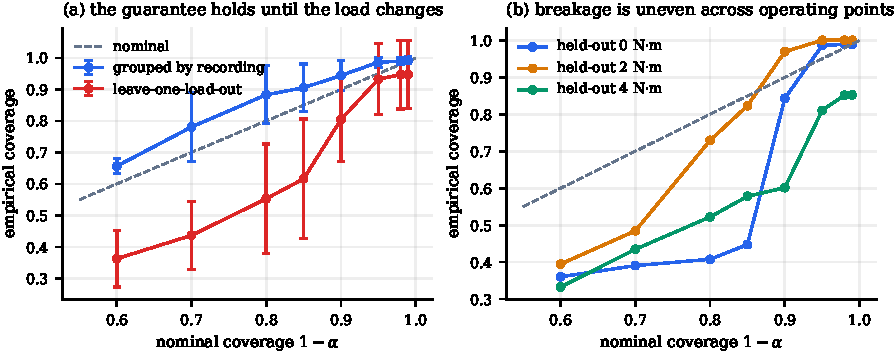
\includegraphics[width=\textwidth]{figs/f_coverage.pdf}
\caption{Empirical versus nominal coverage of the LAC conformal sets.
Under recording-grouped validation (a, blue) the guarantee holds and is
conservative. Under leave-one-load-out (a, red) it fails: a nominal 80\%
delivers \covEighty\%. Panel (b) shows the failure is uneven ---
at $\alpha = 0.20$, coverage is \covZero, \covTwo{} and \covFour{} for
held-out 0, 2 and \SI{4}{\newton\meter}. Error bars are one standard
deviation over seeds and classifiers.}
\label{fig:coverage}
\end{figure*}

\subsection{Coverage collapses under operating-point shift}
Fig.~\ref{fig:coverage} is the central result. Under grouped validation
the guarantee behaves exactly as the theory says: mean gap $\gapGrouped$,
conservative, never meaningfully below nominal. Under leave-one-load-out
the mean gap is $\gapLolo$ and the worst case is $\gapLoloWorst$. A
nominal 80\% interval delivers \covEighty\% empirical coverage.

This is not a surprise --- a change of torque load breaks exchangeability
between calibration and test, and the guarantee is conditional on
exchangeability~\cite{tibshirani2019,barber2023}. It is nonetheless the
number a practitioner needs, because the failure is silent: the node keeps
emitting singletons at the same rate, and the meaning of those singletons
has changed. Panel (b) shows the breakage is also uneven across operating
points, so an integrator cannot budget for it with a single safety factor.

\begin{figure}[t]
\centering
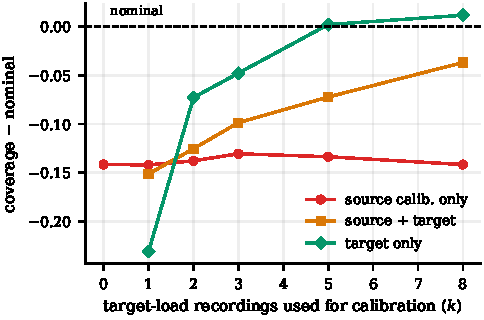
\includegraphics[width=\columnwidth]{figs/f_recal.pdf}
\caption{Recalibration at the target operating point. Five recordings
restore nominal coverage. Pooling the stale source calibration set with
the new one is consistently worse than discarding it.}
\label{fig:recal}
\end{figure}

% GERADO POR make_tables.py -- NAO EDITAR A MAO
\begin{table}[t]
\centering\footnotesize\setlength{\tabcolsep}{5pt}
\caption{Coverage gap (empirical $-$ nominal) after recalibrating with $k$
recordings from the target operating point. Five target recordings restore
nominal coverage --- and \emph{discarding} the source calibration set beats
pooling it at every $k \geq 2$.}
\label{tab:recal}
\begin{tabular}{cccc}
\toprule
$k$ & source only & source $+$ target & target only \\
\midrule
0 & $-0.142$ & -- & -- \\
1 & $-0.142$ & $-0.151$ & $-0.231$ \\
2 & $-0.138$ & $-0.125$ & $-0.073$ \\
3 & $-0.131$ & $-0.099$ & $-0.048$ \\
5 & $-0.134$ & $-0.072$ & \textbf{$+0.002$} \\
8 & $-0.142$ & $-0.037$ & \textbf{$+0.012$} \\
\bottomrule
\end{tabular}
\end{table}


\subsection{What it takes to fix it}
Table~\ref{tab:recal} and Fig.~\ref{fig:recal} quantify recalibration as a
function of the number $k$ of recordings available from the target
operating point. Two findings. First, $k=5$ brings the gap to
$\recalFive$: recalibration is a commissioning procedure with a number
attached, not an open-ended data-collection requirement. Second, and less
intuitively, at $k=3$ recalibrating on target data \emph{alone} gives
$\recalThreeT$ while pooling source and target gives $\recalThreeST$ ---
roughly twice as bad. The stale scores drag the quantile in the wrong
direction. What the quantile needs is exchangeability with the test point,
not sample size, and the natural instinct to keep all available
calibration data is actively harmful here.

% =====================================================================
\section{Discussion and limitations}

% --- CÂNDIDO: NÃO cortes esta seção para ganhar espaço. Ela é metade da
%     razão pela qual o paper é difícil de derrubar.
The honest reading of these results is that a conformal escalation gate is
a better \emph{interface} than a softmax threshold and not a better
\emph{predictor}, and that its guarantee --- the thing that makes it worth
the trouble --- is exactly what breaks first when the machine leaves the
operating point it was calibrated at. The practical consequence is that
conformal gates should be deployed with a recalibration procedure attached,
and we give the size of that procedure.

Limitations. (i) One dataset. The mechanism should be reproduced on at
least one further bench --- we regard this as the first requirement for a
journal version. (ii) 45 recordings, and only three in the normal
condition, which caps the number of grouped folds at three and widens every
interval. (iii) Cost is reported in operations, not joules; the ranking
between cascade designs can change once front-end power is included, and
we deliberately do not claim an energy number we have not measured.
(iv) Load is the only shift we test; speed, temperature and sensor
mounting are all plausible and untested.
\TODO{se conseguires rodar o MAFAULDA antes do prazo, (i) sai daqui e vira
uma subseção de resultados --- é a mudança que mais aumenta a chance de
aceite}

% =====================================================================
\section{Conclusion}
We framed multimodal sensor escalation as a conformal set-size test,
replacing an arbitrary confidence threshold with a stated risk level and
turning the escalation rate into a measured quantity. On the KAIST bearing
dataset the gate matches a tuned softmax threshold in accuracy, and its
coverage guarantee --- valid under recording-grouped validation --- fails
under a change of torque load, delivering \covEighty\% where 80\% was
requested. Five recordings from the target operating point restore the
guarantee, and pooling them with the stale calibration set is worse than
replacing it. We read this as an argument for treating conformal
calibration as a commissioning step tied to the operating point, rather
than a one-off performed in the lab.

% =====================================================================
\bibliographystyle{IEEEtran}   %<<TEMPLATE>> -> IEEEbib
\bibliography{refs}

\end{document}

% =====================================================================
% NOTA SOBRE PRIOR ART -- LER ANTES DE SUBMETER
%
% A checagem de prior art de conformal prediction em PHM / diagnóstico de
% máquinas rotativas AINDA NÃO FOI FEITA. É o único item que pode
% invalidar o enquadramento inteiro deste rascunho.
%
% O que procurar, nesta ordem:
%   1. "conformal prediction" + ("fault diagnosis" | "condition monitoring"
%      | "prognostics" | "remaining useful life")
%   2. cobertura conforme sob mudança de condição de operação / working
%      condition shift -- se isto já foi publicado em PHM, a Seção 4.3
%      deixa de ser contribuição e vira confirmação, e o paper tem de se
%      reposicionar no conserto (Seção 4.4) e no portão (Seção 2.2).
%   3. escalonamento hierárquico / wake-up de sensores com incerteza
%      calibrada -- para o related work da cascata.
%
% Se (2) já existir: o paper não morre, mas o abstract e a lista de
% contribuições têm de ser reescritos com a Seção 4.4 na frente.
% =====================================================================
